\section{Vetores}\label{vetores}

São representados por segmentos orientados e são caracterizados por

\begin{enumerate}
\def\labelenumi{\arabic{enumi}.}
\itemsep1pt\parskip0pt\parsep0pt
\item
  Módulo
\item
  Direção
\item
  Sentido
\end{enumerate}

O módulo de um vetor $\vec{u} = (u_1, u_2)$ é dado por:

\[
|\vec{u}| = \sqrt{u_1^2 + u_2^2}
\]

\subsection{Soma de Vetores}\label{soma-de-vetores}

O resultado é um outro vetor com origem na origem do primeiro e
extremidade na extremidade do último.

\subsubsection{Propriedades da Soma}\label{propriedades-da-soma}

\paragraph{Comutatividade}\label{comutatividade}

\[
\vec{v} + \vec{w} = \vec{w} + \vec{v}
\]

\paragraph{Associatividade}\label{associatividade}

\[
\vec{u} + (\vec{v} + \vec{w}) = (\vec{u} + \vec{v}) + \vec{w}
\]

\paragraph{Existência do elemento
Neutro}\label{existuxeancia-do-elemento-neutro}

\[
\vec{v} + 0 = 0 + \vec{v} = \vec{v}
\]

\paragraph{Existência do elemento inverso da
soma}\label{existuxeancia-do-elemento-inverso-da-soma}

\[
\vec{v} + (-\vec{v}) = 0
\]

\subsection{Multiplicação de um vetor por um
escalar}\label{multiplicauxe7uxe3o-de-um-vetor-por-um-escalar}

Seja $\alpha$ um número real não-nulo e $\vec{v}$ um vetor. Dizemos que
$\alpha \vec{v}$:

\begin{enumerate}
\def\labelenumi{\arabic{enumi}.}
\itemsep1pt\parskip0pt\parsep0pt
\item
  Módulo: $|\alpha|$
\item
  Direção: mesma de $\vec{v}$
\item
  Sentido:

  \begin{itemize}
  \itemsep1pt\parskip0pt\parsep0pt
  \item
    mesmo sentido de $\vec{v}$ se $\alpha > 0$
  \item
    sentido oposto caso contrário
  \end{itemize}
\end{enumerate}

\subsubsection{Propriedades da multiplicação por
escalar}\label{propriedades-da-multiplicauxe7uxe3o-por-escalar}

\paragraph{Associatividade}\label{associatividade-1}

\[
\alpha (\beta \vec{v}) = (\alpha \beta) \vec{v}
\]

\paragraph{Distributividade}\label{distributividade}

\[
\alpha (\vec{v} + \vec{w}) = \alpha \vec{v} + \alpha \vec{w}
\]

\[
(\alpha + \beta) \vec{v} = \alpha \vec{v} + \beta \vec{v}
\]

\subsection{Produto Escalar}\label{produto-escalar}

Também conhecido como Produto Interno, é denotado por
$\vec{v} \cdot \vec{w}$, e definido por

\[
\vec{v} \cdot \vec{w} = v_1 w_1 + v_2 w_2
\]

Quando $\vec{v}$ e $\vec{w}$ são vetores no plano, e

\[
\vec{v} \cdot \vec{w} = v_1 w_1 + v_2 w_2 + v_3 w_3
\]

Quando $\vec{v}$ e $\vec{w}$ são vetores no espaço.

\subsubsection{Teorema}\label{teorema}

\[
\vec{v} \cdot \vec{w} = |\vec{v}| |\vec{w}| \cos \theta
\]

Onde $\theta$ é o ângulo entre estes vetores.

Daí temos também que

\[
\cos \theta = \frac{\vec{v} \cdot \vec{w}}{|\vec{v}| |\vec{w}|}
\]

\subsubsection{Direção de um Vetor Cartesiano
3D}\label{direuxe7uxe3o-de-um-vetor-cartesiano-3d}

Seja um vetor $\vec{u} = (u_1, u_2, u_3)$. Para determinar o ângulo
$\alpha$ que o vetor $\vec{u}$ faz com o $x$ basta fazer:

\[
\cos \alpha = \frac{u_1}{|\vec{u}|} = \frac{u_1}{\sqrt{u_1^2 + u_2^2 + u_3^2}}
\]

O mesmo vale para os outros eixos:

\[
\cos \beta = \frac{u_2}{|\vec{u}|}
\]

\[
\cos \gamma = \frac{u_3}{|\vec{u}|}
\]

\textbf{OBS.:} para chegar a este resultado basta fazer o produto
escalar de $\vec{u}$ por um vetor unitário.

\subsubsection{Propriedades do Produto
Escalar}\label{propriedades-do-produto-escalar}

\paragraph{Comutatividade}\label{comutatividade-1}

\[
\vec{v} \cdot \vec{w} = \vec{w} \cdot \vec{v}
\]

\paragraph{Distributividade}\label{distributividade-1}

\[
\vec{u} \cdot (\vec{v} + \vec{w}) = \vec{u} \cdot \vec{v} + \vec{u} \cdot \vec{w}
\]

\paragraph{Multiplicação por
escalar}\label{multiplicauxe7uxe3o-por-escalar}

\[
\alpha (\vec{v} \cdot \vec{w}) = (\alpha \vec{v}) \cdot \vec{w} = \vec{v} \cdot (\alpha \vec{w})
\]

\subsection{Produto Vetorial}\label{produto-vetorial}

É denotado por $\vec{v} \times \vec{w}$, e definido por

\[
|\vec{v} \times \vec{w}| = |\vec{v}| |\vec{w}| \sin \theta
\]

Direção: perpendicular ao plano determinado por $\vec{v}$ e $\vec{w}$

\subsubsection{Propriedades do Produto
Vetorial}\label{propriedades-do-produto-vetorial}

\paragraph{Anticomutatividade}\label{anticomutatividade}

\[
\vec{v} \times \vec{w} = - \vec{w} \times \vec{v}
\]

\paragraph{Distributividade}\label{distributividade-2}

\[
\vec{u} \times (\vec{v} + \vec{w}) = \vec{u} \times \vec{v} + \vec{u} \times \vec{w}
\]

\paragraph{Multiplicação por
escalar}\label{multiplicauxe7uxe3o-por-escalar-1}

\[
\alpha (\vec{v} \times \vec{w}) = (\alpha \vec{v}) \times \vec{w} = \vec{v} \times (\alpha \vec{w})
\]

\subsubsection{Teorema 1}\label{teorema-1}

Sejam $\vec{v} = (v_1, v_2, v_3)$ e $\vec{w} = (w_1, w_2, w_3)$. Então

\[
\vec{v} \times \vec{w}
= \det
\begin{vmatrix}
i & j & k \\
v_1 & v_2 & v_3 \\
w_1 & w_2 & w_3
\end{vmatrix}
\]

\section{Cargas Elétricas}\label{cargas-eluxe9tricas}

\subsection{Definições Gerais}\label{definiuxe7uxf5es-gerais}

\paragraph{Condutores}\label{condutores}

São materiais nos quais as cargas elétricas se movem com facilidade.

\paragraph{Isolantes}\label{isolantes}

São materiais nos quais as cargas elétricas não podem se mover.

\paragraph{Semicondutores}\label{semicondutores}

São materiais com propriedades elétricas intermediárias entre as dos
condutores e as dos isolantes.

\paragraph{Supercondutores}\label{supercondutores}

São condutores perfeitos, ou seja, em que as cargas se movem sem
encontrar nenhuma resistência.

\paragraph{Força eletroestática}\label{foruxe7a-eletroestuxe1tica}

Força de repulsão ou atração associada à carga elétrica.

Se as cargas das partículas tem o mesmo sinal, elas se repelem. Caso
tenham sinais opostos, elas se atraem.

\subsection{Lei de Coulomb}\label{lei-de-coulomb}

Permite calcular a força exercida por partículas carregadas.

\[
\vec{F} = k \frac{q_1 \cdot q_2}{r^2} \hat{r}
\]

onde $\hat{r}$ é um vetor unitário na direção da reta que liga as duas
partículas, $r$ é a distância entre as partículas e $k$ é uma constante,
com valor $1/4 \pi \varepsilon_0$.

Rescrevendo temos:

\[
F = \frac{1}{4 \pi \varepsilon_0} \frac{|q_1| \cdot |q_2|}{r^2}
\]

Podemos também substituir:

\[
k = \frac{1}{4 \pi \varepsilon_0} = 8,99 \times 10^9 N \cdot m^2/C^2
\]

A constante $\varepsilon_0$, conhecida como \textbf{permissividade do
vácuo}, tem o valor:

\[
\varepsilon_0 = 8,85 \times 10^{-12} C^2/N \cdot m^2
\]

\subsection{Cascas Esféricas}\label{cascas-esfuxe9ricas}

\paragraph{Teorema 1}\label{teorema-1-1}

Uma casca com uma distribuição uniforme de carga atrai ou repele uma
partícula carregada situada do lado de fora da casca como se toda a
carga da casca estivesse situada no centro.

\paragraph{Teorema 2}\label{teorema-2}

Se uma partícula carregada está situada no interior de uma casca com uma
distribuição uniforme de carga, a casca não exerce nehuma força
eletroestática sobre a partícula.

\subsection{Quantidade de carga}\label{quantidade-de-carga}

\[
q = n \cdot e
\]

onde $e$, a \textbf{carga elementar}, tem valor aproximado

\[
e = 1,602 \times 10^{-19} C
\]

\section{Campo Elétrico}\label{campo-eluxe9trico}

\subsection{Carga de Prova}\label{carga-de-prova}

\paragraph{Definição}\label{definiuxe7uxe3o}

É uma carga imaginária de tamanho infinitesimal que não gera campo e é
sempre positiva.

\subsection{Direção do campo}\label{direuxe7uxe3o-do-campo}

\paragraph{Afastamento}\label{afastamento}

Se ao colocar uma carga de prova aparecer uma força de afastamento.

\paragraph{Atração}\label{atrauxe7uxe3o}

Se ao colocar uma carga de prova aparecer uma força de atração.

\subsection{Intensidade (Módulo) do
Campo}\label{intensidade-muxf3dulo-do-campo}

é definido como o quociente entre as forças de interação das cargas
geradora do campo ($Q$) e de prova ($q$) e a própria carga de prova
($q$), ou seja:

\[
E = \frac{F}{q} \Rightarrow \frac{k \cdot \frac{Q \cdot q}{d^2}}{q}
  \Rightarrow k \cdot \frac{Q}{d^2}
\]

\paragraph{Unidade}\label{unidade}

N/C - Newton por Coulomb

\subsection{Dipolo elétrico}\label{dipolo-eluxe9trico}

é formado por duas partículas com cargas de mesmo valor absoluto $q$ e
sinais opostos, separadas por uma pequena distância $d$.

O módulo do campo elétrico de um dipolo em um ponto distante sobre o
eixo do dipolo é dado por:

\[
E = \frac{1}{2 \pi \varepsilon_0} \frac{p}{z^3}
\]

onde $p = q \cdot d$, e $z$ é a distância entre o ponto e o centro do
dipolo.

\subsection{Campo elétrico produzido por uma linha de
cargas}\label{campo-eluxe9trico-produzido-por-uma-linha-de-cargas}

\paragraph{Módulo de uma anel
carregado}\label{muxf3dulo-de-uma-anel-carregado}

\[
E = \frac{q \cdot z}{4 \pi \varepsilon_0 (z^2 + R^2)^\frac{3}{2}}
\]

onde $z$ é a distância entre o centro do anel ao ponto $P$. O raio do
anel é $R$.

\paragraph{Módulo de um disco
carregado}\label{muxf3dulo-de-um-disco-carregado}

\[
E = \frac{\sigma}{2 \varepsilon_0}(1 - \frac{z}{\sqrt{z^2 + R^2}})
\]

onde $\sigma$ é a carga por unidade de área, e $z$ é a distância entre o
centro do disco ao ponto $P$. O raio do disco é $R$.

\section{Apêndice A}\label{apuxeandice-a}

\subsection{Comprimento, Área e
Volume}\label{comprimento-uxe1rea-e-volume}

\paragraph{Comprimento do círculo}\label{comprimento-do-cuxedrculo}

\[
C = 2 \cdot \pi \cdot r
\]

\paragraph{Área do círculo}\label{uxe1rea-do-cuxedrculo}

\[
A = \pi \cdot r^2
\]

\paragraph{Área do trapézio}\label{uxe1rea-do-trapuxe9zio}

\[
A = \frac{h \cdot (B + b)}{2}
\]

\paragraph{Volume da esfera}\label{volume-da-esfera}

\[
V = \frac{4 \cdot \pi r^3}{3}
\]

\paragraph{Volume do cubo}\label{volume-do-cubo}

\[
V = a^3 \text{\, onde $a$ é a aresta}
\]

\paragraph{Volume do cone circular
reto}\label{volume-do-cone-circular-reto}

\[
V = \frac{\pi \cdot r^2 \cdot h}{3}
\]

\paragraph{Volume da pirâmide}\label{volume-da-piruxe2mide}

\[
V = \frac{A_b \cdot h}{3} \text{\, onde $A_b$ é a área da base}
\]

\subsection{Trigonometria}\label{trigonometria}

Relações trigonométricas seno, cosseno e tangente.

\begin{longtable}[c]{@{}lccc@{}}
\toprule\addlinespace
\begin{minipage}[b]{0.12\columnwidth}\raggedright
~
\end{minipage} & \begin{minipage}[b]{0.26\columnwidth}\centering
30
\end{minipage} & \begin{minipage}[b]{0.26\columnwidth}\centering
45
\end{minipage} & \begin{minipage}[b]{0.26\columnwidth}\centering
60
\end{minipage}
\\\addlinespace
\midrule\endhead
\begin{minipage}[t]{0.12\columnwidth}\raggedright
seno
\end{minipage} & \begin{minipage}[t]{0.26\columnwidth}\centering
$\frac{1}{2}$
\end{minipage} & \begin{minipage}[t]{0.26\columnwidth}\centering
$\frac{\sqrt{2}}{2}$
\end{minipage} & \begin{minipage}[t]{0.26\columnwidth}\centering
$\frac{\sqrt{3}}{2}$
\end{minipage}
\\\addlinespace
\begin{minipage}[t]{0.12\columnwidth}\raggedright
cosseno
\end{minipage} & \begin{minipage}[t]{0.26\columnwidth}\centering
$\frac{\sqrt{3}}{2}$
\end{minipage} & \begin{minipage}[t]{0.26\columnwidth}\centering
$\frac{\sqrt{2}}{2}$
\end{minipage} & \begin{minipage}[t]{0.26\columnwidth}\centering
$\frac{1}{2}$
\end{minipage}
\\\addlinespace
\begin{minipage}[t]{0.12\columnwidth}\raggedright
tangente
\end{minipage} & \begin{minipage}[t]{0.26\columnwidth}\centering
$\frac{\sqrt{3}}{3}$
\end{minipage} & \begin{minipage}[t]{0.26\columnwidth}\centering
$1$
\end{minipage} & \begin{minipage}[t]{0.26\columnwidth}\centering
$\sqrt{3}$
\end{minipage}
\\\addlinespace
\bottomrule
\end{longtable}

Para um triângulo retângulo como visto na figura:

\begin{figure}[htbp]
\centering
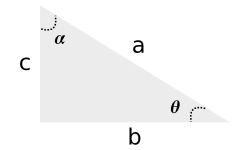
\includegraphics{img/triangulo-retangulo.jpg}
\caption{Triângulo Retângulo}
\end{figure}

Teorema de Pitágoras:

\[
a^2 = b^2 + c^2
\]

As funções seno e cosseno são definidas como:

\[
\sin \theta = \frac{\text{CO}}{\text{H}} = \frac{c}{a} = \cos \alpha
\]

\[
\cos \theta = \frac{\text{CA}}{\text{H}} = \frac{b}{a} = \sin \alpha
\]

\[
\sin^2 \theta + \cos^2 \theta = 1
\]
